\documentclass[12pt]{article}

\usepackage[margin=0.5in]{geometry}
\usepackage{tikz}
\newcommand{\wht}[3]{
\draw[fill=white] (#1,#2) circle (0.45);
\node at (#1,#2) {#3};}
\newcommand{\blk}[3]{
\draw[fill=black] (#1,#2) circle (0.45);
\node[text=white] at (#1,#2) {#3};}


\title{\textbf{Problem Set} 10 April 2018}
\date{}
\begin{document}

\sffamily

\maketitle

% EXERCISES #1 & #2
\noindent 
\parbox[t]{0.5\textwidth}{\textbf{Joseki 01}  \\ \\
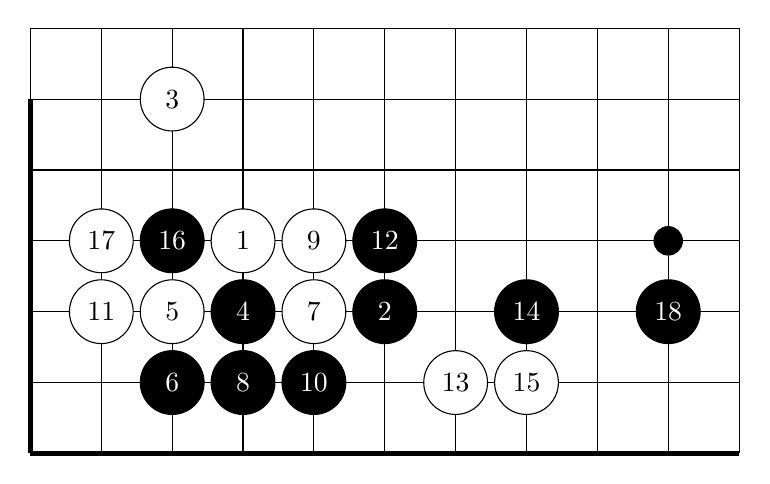
\begin{tikzpicture}[scale=0.9]
\draw[line width=2] (0,0)--(10,0);
\draw[line width=2] (0,0)--(0,5);
\foreach \a in {0,...,6}{
	\draw (0,\a)--(10,\a);
}
\foreach \a in {0,...,10}{
	\draw (\a,0)--(\a,6);
}
\draw[fill=black] (3,3) circle (0.2);
\draw[fill=black] (9,3) circle (0.2);

\wht{3}{3}{1}
\blk{5}{2}{2}
\wht{2}{5}{3}
\blk{3}{2}{4}
\wht{2}{2}{5}
\blk{2}{1}{6}
\wht{4}{2}{7}
\blk{3}{1}{8}
\wht{4}{3}{9}
\blk{4}{1}{10}
\wht{1}{2}{11}
\blk{5}{3}{12}
\wht{6}{1}{13}
\blk{7}{2}{14}
\wht{7}{1}{15}
\blk{2}{3}{16}
\wht{1}{3}{17}
\blk{9}{2}{18}

\end{tikzpicture} \\
I've personally never seen Black 4, so we put down \\ a continuation to 16 moves, as played in the game.
\vfill
}% <--------- no space
\parbox[t]{0.5\textwidth}{\textbf{Joseki 02}  \\ \\
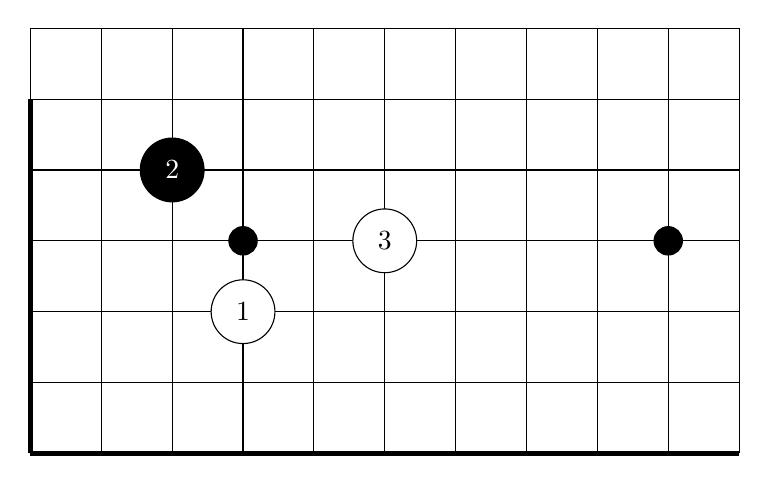
\begin{tikzpicture}[scale=0.9]
\draw[line width=2] (0,0)--(10,0);
\draw[line width=2] (0,0)--(0,5);
\foreach \a in {0,...,6}{
	\draw (0,\a)--(10,\a);
}
\foreach \a in {0,...,10}{
	\draw (\a,0)--(\a,6);
}
\draw[fill=black] (3,3) circle (0.2);
\draw[fill=black] (9,3) circle (0.2);
\wht{3}{2}{1}
\blk{2}{4}{2}
\wht{5}{3}{3}
\end{tikzpicture} \\
A 3-4 variant. }

\vspace{6pt}

\hrule

\vspace{6pt}

% EXERCISES #3 & #4
\noindent
\parbox[t]{0.5\textwidth}{\textbf{Exercise 03}  \\ \\
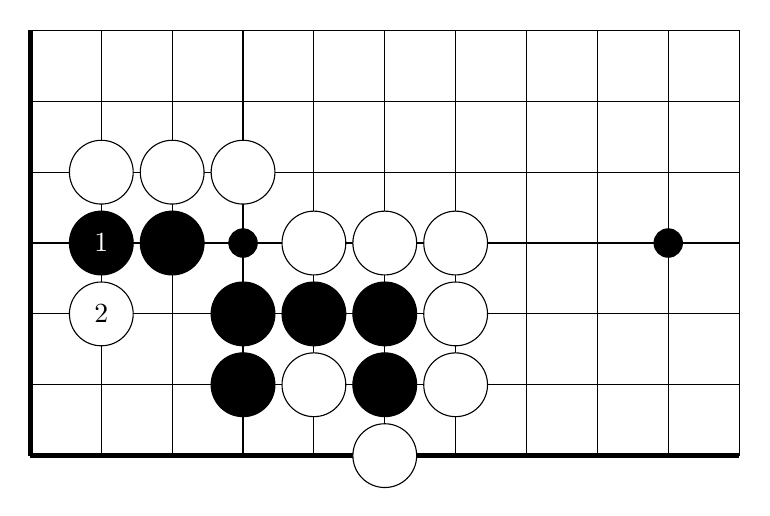
\begin{tikzpicture}[scale=0.9]
\draw[line width=2] (0,0)--(10,0);
\draw[line width=2] (0,0)--(0,6);
\foreach \a in {0,...,6}{
	\draw (0,\a)--(10,\a);
}
\foreach \a in {0,...,10}{
	\draw (\a,0)--(\a,6);
}
\draw[fill=black] (3,3) circle (0.2);
\draw[fill=black] (9,3) circle (0.2);

\blk{1}{3}{1}
\wht{1}{2}{2}

\wht{1}{4}{}
\wht{2}{4}{}
\wht{3}{4}{}
%\wht{3}{3}{}
\wht{4}{3}{}
\wht{5}{3}{}
\wht{6}{3}{}
\wht{6}{2}{}
\wht{6}{1}{}
\wht{5}{0}{}
\wht{4}{1}{}

\blk{5}{1}{}
\blk{5}{2}{}
\blk{4}{2}{}
\blk{3}{2}{}
\blk{3}{1}{}
\blk{2}{3}{}

\end{tikzpicture} \\
Does Black have enough room to surivive without ko?
}% <---- no space
\parbox[t]{0.5\textwidth}{\textbf{Exercise 04}  \\ \\
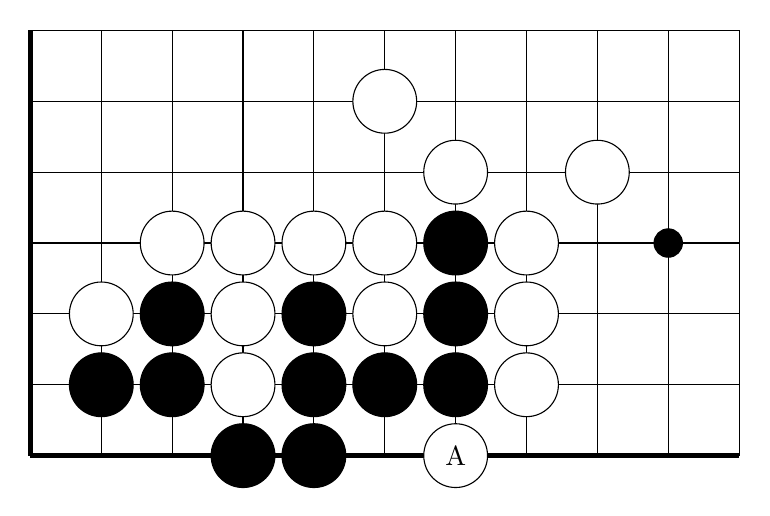
\begin{tikzpicture}[scale=0.9]
\draw[line width=2] (0,0)--(10,0);
\draw[line width=2] (0,0)--(0,6);
\foreach \a in {0,...,6}{
	\draw (0,\a)--(10,\a);
}
\foreach \a in {0,...,10}{
	\draw (\a,0)--(\a,6);
}
\draw[fill=black] (3,3) circle (0.2);
\draw[fill=black] (9,3) circle (0.2);

\blk{1}{1}{}
\blk{2}{1}{}
\blk{2}{2}{}
\blk{3}{0}{}
\blk{4}{0}{}
\blk{4}{1}{}
\blk{4}{2}{}
\blk{5}{1}{}
\blk{6}{1}{}
\blk{6}{2}{}
\blk{6}{3}{}

\wht{1}{2}{}
\wht{2}{3}{}
\wht{3}{3}{}
\wht{3}{2}{}
\wht{3}{1}{}
\wht{4}{3}{}
\wht{5}{3}{}
\wht{5}{2}{}
\wht{7}{1}{}
\wht{7}{2}{}
\wht{7}{3}{}
\wht{6}{4}{}
\wht{8}{4}{}
\wht{5}{5}{}

\wht{6}{0}{A}
\end{tikzpicture} \\
Is \textbf{A} the correct move for White?}

\vspace{6pt}

\hrule

\vspace{6pt}

% EXERCISES #5 & #6
\noindent
\parbox[t]{0.5\textwidth}{\textbf{Exercise 05}  \\ \\
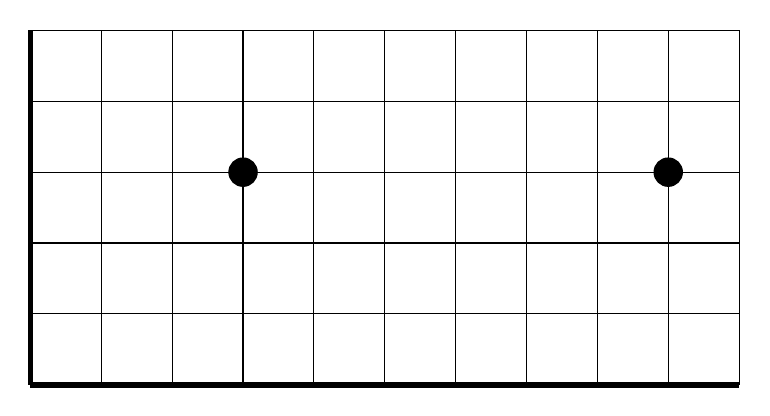
\begin{tikzpicture}[scale=0.9]
\draw[line width=2] (0,0)--(10,0);
\draw[line width=2] (0,0)--(0,5);
\foreach \a in {0,...,5}{
	\draw (0,\a)--(10,\a);
}
\foreach \a in {0,...,10}{
	\draw (\a,0)--(\a,5);
}
\draw[fill=black] (3,3) circle (0.2);
\draw[fill=black] (9,3) circle (0.2);
\end{tikzpicture} \\
What is the next move in this Joseki?
}% <---- no space
\parbox[t]{0.5\textwidth}{\textbf{Exercise 06} \\ \\
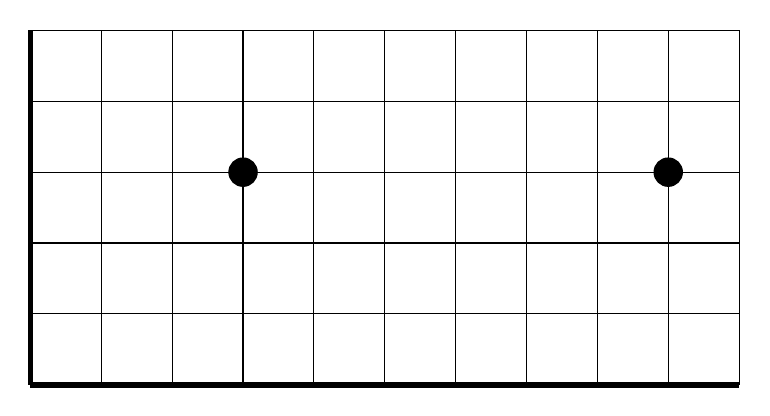
\begin{tikzpicture}[scale=0.9]
\draw[line width=2] (0,0)--(10,0);
\draw[line width=2] (0,0)--(0,5);
\foreach \a in {0,...,5}{
	\draw (0,\a)--(10,\a);
}
\foreach \a in {0,...,10}{
	\draw (\a,0)--(\a,5);
}
\draw[fill=black] (3,3) circle (0.2);
\draw[fill=black] (9,3) circle (0.2);
\end{tikzpicture} \\
What is the next move in this Joseki? }



\end{document}